\documentclass{standalone}


\usepackage{tikz}

\begin{document}
	
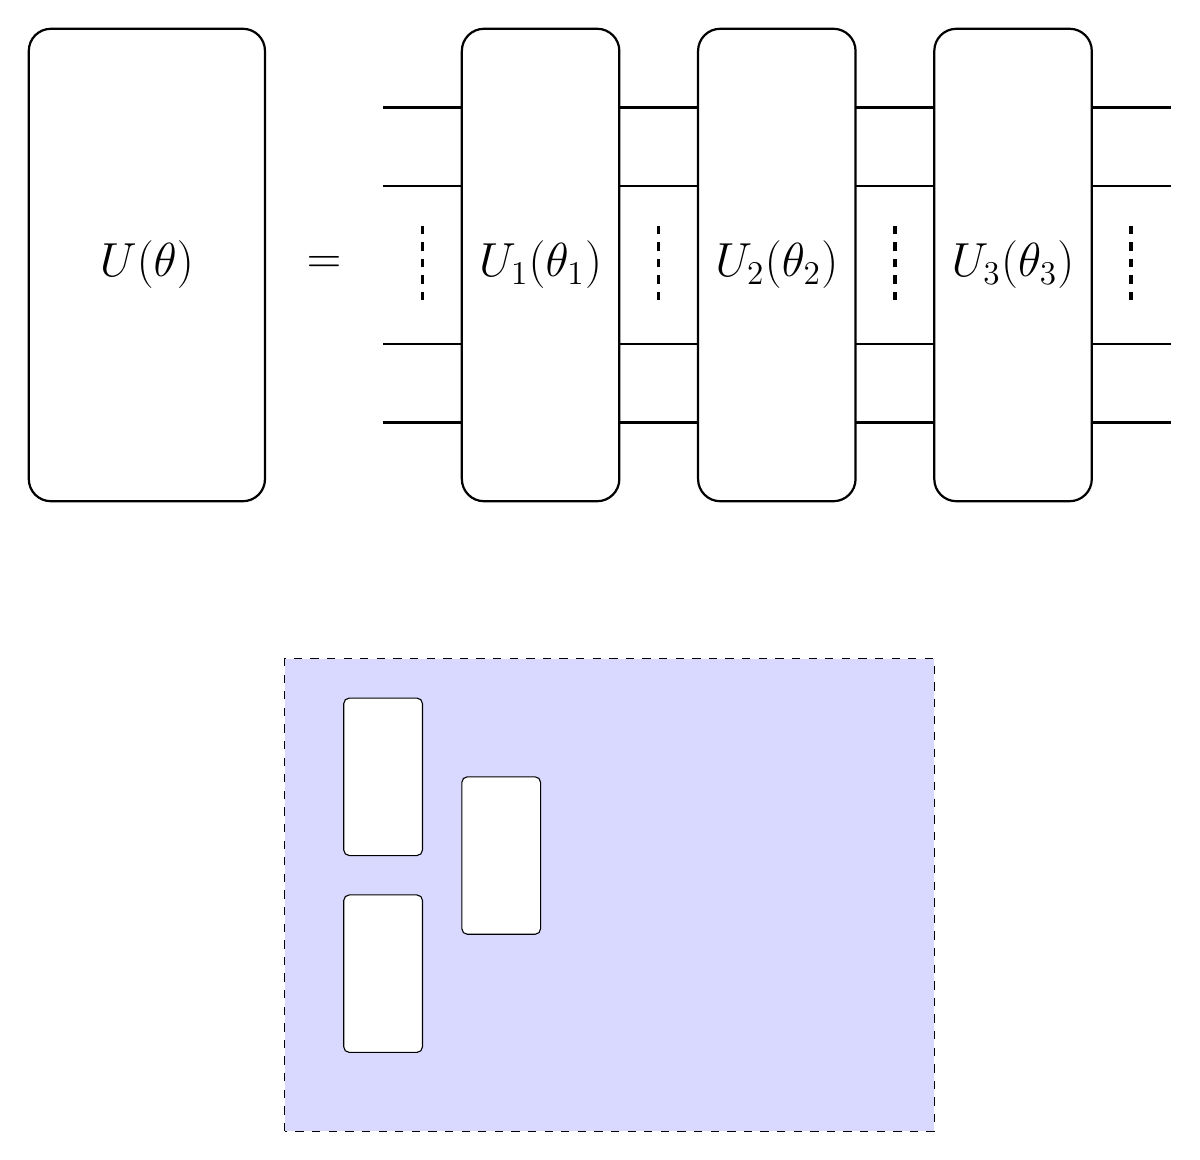
\begin{tikzpicture}
%	\draw (2,0) -- (-1,2);
%	\draw (0,0) circle [radius=10pt];
%	\draw  [<->](0,0.25) -- (0.5,1.2);
%	\draw (0,0) rectangle (0.5,1);
%	\draw[step=.5cm] (-2,-2) grid (2,2);
%   \draw [<->] (0,0) arc [start angle=180, end angle=30, radius=10pt];
%	\tikz \foreach \x in {3,5,7}
%		\draw (\x,0) rectangle (\x,2);
%\draw[thick,rounded corners=8pt]
%										(0,0) -- (2,1);

	\tikzstyle{operator} = [fill=white,minimum size=1.5em]
	\tikzstyle{ctrl} = [fill,shape=circle,minimum size=5pt,inner sep=0pt]
	\tikzstyle{tgrt} = [shape=circle,minimum size=5pt,inner sep=0pt]

	\draw[thick,rounded corners=8pt,fill=white] (-2.5,0) rectangle (-2.5+3,6);
	\node [anchor=center] at (-1,3) {\LARGE $U(\theta)$};
	
	\node [anchor=center] at (1.25,3) {\LARGE $=$};

	\foreach \x [evaluate=\x] in {3,6,9,12} 
	\draw[very thick,dash pattern=on 3pt off 3pt] (\x-0.5,3.5) -- (\x-0.5,2.5);

	\foreach \x [evaluate=\x] in {3,6,9} {
		\foreach \y in {1,2,4,5}
			\draw[thick] (\x-1,\y) -- (\x+3,\y);
		}

	\foreach \x  [evaluate=\x] in {1,2,3} {
		\draw[thick,rounded corners=8pt,fill=white] (3*\x,0) rectangle (3*\x+2,6);
		\node [anchor=center] at (3*\x+1,3) { \LARGE $U_\x(\theta_\x)$};
	}


	\draw[dashed,fill=blue!15] (5.75-5,-8) rectangle (5.75+3.25,-2);
	

\begin{scope}[shift={(1.5,-4.5)}]
		\draw[thin,rounded corners=2pt,fill=white] (0,0) rectangle (1,2);
		\draw[thin,rounded corners=2pt,fill=white] (0,-0.5) rectangle (1,-2.5);
		\draw[thin,rounded corners=2pt,fill=white] (1.5,1) rectangle (2.5,-1);
		
\end{scope}

\end{tikzpicture}
\end{document}